\section{Supplementary pooling, metrics, and uncertainty}
\label{sec:supplement}
The supplementary \meanmodel{} uses seeds 42, 44, and 2026, the same five development folds, observed-history protocol, future-state objective, and forecast feature groups as \fullmodel{}, replacing spatial attention with mean pooling. Metrics are computed from patient-wise five-fold probability means within each seed and then averaged across the three seeds. The per-seed results in Table~\ref{tab:seedresults} preserve the individual training realizations underlying the reported mean and sample standard deviation.
\begin{table*}[t]
\centering
\small
\caption{Supplementary spatial pooling comparison, mean $\pm$ sample SD over seeds 42,44,2026. Within-seed fivefold probabilities are averaged before metrics, then seed metrics are averaged. ForecastMean and ForecastAttention share forecast readout and future-state supervision.}
\label{tab:pooling}
\begin{tabular}{llrrr}
\toprule
Model & Landmark & AUROC & AP & F1 \\
\midrule
ForecastMean & T0 & 0.7451 $\pm$ 0.0040 & 0.6093 $\pm$ 0.0093 & 0.5677 $\pm$ 0.0047 \\
ForecastMean & T1 & 0.7465 $\pm$ 0.0051 & 0.6137 $\pm$ 0.0028 & 0.5785 $\pm$ 0.0161 \\
ForecastMean & T2 & 0.7446 $\pm$ 0.0049 & 0.6166 $\pm$ 0.0044 & 0.5707 $\pm$ 0.0033 \\
ForecastMean & Macro & 0.7454 $\pm$ 0.0043 & 0.6132 $\pm$ 0.0048 & 0.5723 $\pm$ 0.0048 \\
ForecastAttention & T0 & 0.7437 $\pm$ 0.0025 & 0.6166 $\pm$ 0.0079 & 0.5547 $\pm$ 0.0185 \\
ForecastAttention & T1 & 0.7460 $\pm$ 0.0053 & 0.6170 $\pm$ 0.0101 & 0.5507 $\pm$ 0.0141 \\
ForecastAttention & T2 & 0.7464 $\pm$ 0.0074 & 0.6170 $\pm$ 0.0127 & 0.5615 $\pm$ 0.0197 \\
ForecastAttention & Macro & 0.7454 $\pm$ 0.0047 & 0.6169 $\pm$ 0.0102 & 0.5556 $\pm$ 0.0143 \\
\bottomrule
\end{tabular}
\end{table*}

\begin{table*}[t]
\centering
\small
\caption{Individual-seed results: patient-level fivefold probability ensembles, each evaluated on the same 175 patients (56 positive). Macro is the mean of three landmark metrics. These seed-specific estimates generate the main table mean and sample SD; they are not independent patient cohorts.}
\label{tab:seedresults}
\begin{tabular}{llrrrr}
\toprule
Model & Seed & Landmark & AUROC & AP & F1 \\
\midrule
NoJEPA & 42 & T0 & 0.7216 & 0.5945 & 0.5217 \\
NoJEPA & 42 & T1 & 0.7176 & 0.5966 & 0.5299 \\
NoJEPA & 42 & T2 & 0.7206 & 0.5957 & 0.5378 \\
NoJEPA & 42 & Macro & 0.7199 & 0.5956 & 0.5298 \\
NoJEPA & 44 & T0 & 0.7275 & 0.5954 & 0.5354 \\
NoJEPA & 44 & T1 & 0.7281 & 0.5981 & 0.5426 \\
NoJEPA & 44 & T2 & 0.7281 & 0.5971 & 0.5469 \\
NoJEPA & 44 & Macro & 0.7279 & 0.5968 & 0.5416 \\
NoJEPA & 2026 & T0 & 0.7291 & 0.5933 & 0.5538 \\
NoJEPA & 2026 & T1 & 0.7246 & 0.5921 & 0.5538 \\
NoJEPA & 2026 & T2 & 0.7216 & 0.5894 & 0.5606 \\
NoJEPA & 2026 & Macro & 0.7251 & 0.5916 & 0.5561 \\
DirectReadout & 42 & T0 & 0.7435 & 0.5881 & 0.5321 \\
DirectReadout & 42 & T1 & 0.7461 & 0.6119 & 0.5487 \\
DirectReadout & 42 & T2 & 0.7389 & 0.5914 & 0.5600 \\
DirectReadout & 42 & Macro & 0.7428 & 0.5971 & 0.5469 \\
DirectReadout & 44 & T0 & 0.7372 & 0.6025 & 0.5669 \\
DirectReadout & 44 & T1 & 0.7416 & 0.6115 & 0.5692 \\
DirectReadout & 44 & T2 & 0.7410 & 0.6086 & 0.5672 \\
DirectReadout & 44 & Macro & 0.7399 & 0.6075 & 0.5678 \\
DirectReadout & 2026 & T0 & 0.7224 & 0.5991 & 0.5246 \\
DirectReadout & 2026 & T1 & 0.7216 & 0.5997 & 0.5085 \\
DirectReadout & 2026 & T2 & 0.7251 & 0.6069 & 0.5469 \\
DirectReadout & 2026 & Macro & 0.7230 & 0.6019 & 0.5266 \\
ForecastAttention & 42 & T0 & 0.7408 & 0.6130 & 0.5366 \\
ForecastAttention & 42 & T1 & 0.7423 & 0.6156 & 0.5410 \\
ForecastAttention & 42 & T2 & 0.7426 & 0.6115 & 0.5410 \\
ForecastAttention & 42 & Macro & 0.7419 & 0.6134 & 0.5395 \\
ForecastAttention & 44 & T0 & 0.7450 & 0.6256 & 0.5736 \\
ForecastAttention & 44 & T1 & 0.7521 & 0.6278 & 0.5442 \\
ForecastAttention & 44 & T2 & 0.7550 & 0.6315 & 0.5634 \\
ForecastAttention & 44 & Macro & 0.7507 & 0.6283 & 0.5604 \\
ForecastAttention & 2026 & T0 & 0.7453 & 0.6111 & 0.5538 \\
ForecastAttention & 2026 & T1 & 0.7437 & 0.6077 & 0.5669 \\
ForecastAttention & 2026 & T2 & 0.7417 & 0.6079 & 0.5802 \\
ForecastAttention & 2026 & Macro & 0.7436 & 0.6089 & 0.5670 \\
ForecastMean & 42 & T0 & 0.7425 & 0.6188 & 0.5714 \\
ForecastMean & 42 & T1 & 0.7407 & 0.6170 & 0.5891 \\
ForecastMean & 42 & T2 & 0.7389 & 0.6168 & 0.5672 \\
ForecastMean & 42 & Macro & 0.7407 & 0.6175 & 0.5759 \\
ForecastMean & 44 & T0 & 0.7431 & 0.6088 & 0.5625 \\
ForecastMean & 44 & T1 & 0.7494 & 0.6121 & 0.5865 \\
ForecastMean & 44 & T2 & 0.7471 & 0.6209 & 0.5736 \\
ForecastMean & 44 & Macro & 0.7465 & 0.6139 & 0.5742 \\
ForecastMean & 2026 & T0 & 0.7497 & 0.6002 & 0.5692 \\
ForecastMean & 2026 & T1 & 0.7495 & 0.6120 & 0.5600 \\
ForecastMean & 2026 & T2 & 0.7477 & 0.6121 & 0.5714 \\
ForecastMean & 2026 & Macro & 0.7490 & 0.6081 & 0.5669 \\
\bottomrule
\end{tabular}
\end{table*}

\begin{table*}[t]
\centering
\footnotesize
\setlength{\tabcolsep}{5pt}
\caption{All 14 macro metrics for the principal variants: point estimate [95\% patient-bootstrap percentile interval]. Within each of seeds 42,44,2026, five fold probabilities are averaged per patient, metrics are computed and averaged over T0--T2, then seed metrics are equally averaged. Threshold-dependent metrics use 0.5. Identical patient resamples preserve pairing across models and landmarks. Entries are marginal model intervals; paired differences are reported separately. Intervals condition on the fitted ensembles and exclude retraining and retrospective selection uncertainty. Downward arrows identify metrics for which lower is better.}
\label{tab:extended_macro}
\begin{tabular}{lccc}
\toprule
Metric & NoJEPA & DirectReadout & ForecastAttention \\
\midrule
AUROC & 0.7243 [0.6401, 0.7989] & 0.7353 [0.6514, 0.8084] & 0.7454 [0.6623, 0.8163] \\
AP & 0.5947 [0.4720, 0.7084] & 0.6022 [0.4818, 0.7169] & 0.6169 [0.4931, 0.7303] \\
F1 & 0.5425 [0.4353, 0.6353] & 0.5471 [0.4416, 0.6414] & 0.5556 [0.4514, 0.6452] \\
Accuracy & 0.6730 [0.6057, 0.7359] & 0.6825 [0.6152, 0.7454] & 0.6692 [0.5994, 0.7314] \\
Sensitivity & 0.6071 [0.4879, 0.7284] & 0.6012 [0.4843, 0.7189] & 0.6468 [0.5273, 0.7659] \\
Specificity & 0.7040 [0.6224, 0.7788] & 0.7208 [0.6431, 0.7935] & 0.6797 [0.5968, 0.7574] \\
PPV & 0.4921 [0.3767, 0.6023] & 0.5053 [0.3878, 0.6175] & 0.4894 [0.3792, 0.5961] \\
NPV & 0.7926 [0.7120, 0.8672] & 0.7943 [0.7145, 0.8677] & 0.8042 [0.7240, 0.8767] \\
Balanced accuracy & 0.6556 [0.5822, 0.7256] & 0.6610 [0.5869, 0.7336] & 0.6633 [0.5893, 0.7312] \\
MCC & 0.2976 [0.1563, 0.4355] & 0.3105 [0.1677, 0.4487] & 0.3096 [0.1689, 0.4404] \\
Youden index & 0.3112 [0.1645, 0.4512] & 0.3220 [0.1738, 0.4672] & 0.3266 [0.1787, 0.4624] \\
NLL $\downarrow$ & 0.5839 [0.5285, 0.6435] & 0.5763 [0.5203, 0.6375] & 0.5823 [0.5336, 0.6363] \\
Brier score $\downarrow$ & 0.2008 [0.1760, 0.2274] & 0.1977 [0.1729, 0.2245] & 0.1998 [0.1778, 0.2237] \\
ECE $\downarrow$ & 0.1193 [0.0901, 0.1854] & 0.1215 [0.0960, 0.1853] & 0.1348 [0.1006, 0.1984] \\
\bottomrule
\end{tabular}
\end{table*}

\begin{table*}[t]
\centering
\small
\caption{Threshold sensitivity analysis: three-seed mean Macro metrics. Each seed uses landmark-specific Youden thresholds from its disjoint validation-fold scores. OOF single-model scores differ from test fivefold ensemble scores; this is sensitivity analysis, not independent ensemble calibration. No test labels choose thresholds.}
\label{tab:extended_threshold}
\begin{tabular}{llrrrr}
\toprule
Model & Policy & F1 & Sens. & Spec. & MCC \\
\midrule
NoJEPA & 0.5 & 0.543 & 0.607 & 0.704 & 0.298 \\
NoJEPA & OOF validation Youden & 0.547 & 0.635 & 0.679 & 0.298 \\
\midrule
DirectReadout & 0.5 & 0.547 & 0.601 & 0.721 & 0.310 \\
DirectReadout & OOF validation Youden & 0.543 & 0.587 & 0.731 & 0.308 \\
\midrule
ForecastAttention & 0.5 & 0.556 & 0.647 & 0.680 & 0.310 \\
ForecastAttention & OOF validation Youden & 0.554 & 0.649 & 0.674 & 0.306 \\
\bottomrule
\end{tabular}
\end{table*}


\subsection{Paired significance checks}
Table~\ref{tab:bootstrap} reports the nine principal Macro comparisons, with unadjusted 95\% paired patient-bootstrap intervals, raw two-sided approximate bootstrap $p$ values, within-family Holm adjustment, and all-90 Holm adjustment. The secondary family comprises 81 tests in Tables~\ref{tab:significance_landmarks}--\ref{tab:significance_longitudinal}. Every patient draw is shared across all three fixed seeds, models, and landmarks; metrics are computed within seeds before averaging. The independent patient count remains 175. A significance marker refers to the stated Holm-adjusted family; ns denotes $p_{\mathrm{Holm}}\geq0.05$. The existing 2,000-resample percentile intervals are unadjusted and are not exact inversions of the 99,999-resample null-centered tests. All testing and reporting choices remain retrospective and exploratory.

\begin{table*}[t]
\centering
\small
\caption{Exploratory landmark comparisons. All metrics use approximate, null-centered paired patient-bootstrap tests (99,999 shared draws across seeds, models, and landmarks). All $p$ values are two-sided. $p_{\mathrm{Holm}}$ adjusts jointly over the 81 secondary tests in Tables~\ref{tab:significance_landmarks}--\ref{tab:significance_longitudinal}. Direct and Attention abbreviate DirectReadout and ForecastAttention. $^{*}p_{\mathrm{Holm}}<0.05$, $^{**}p_{\mathrm{Holm}}<0.01$, $^{***}p_{\mathrm{Holm}}<0.001$; ns, not significant after the stated correction. Intervals are unadjusted 95\% patient-bootstrap intervals (2,000 shared draws) and need not agree with adjusted test decisions. All analyses condition on the fixed, retrospectively selected seed42/44/2026 ensembles; seeds are not resampled.}
\label{tab:significance_landmarks}
\begin{tabular}{lllrrrc}
\toprule
Comparison & Landmark & Metric & Difference [95\% CI] & $p$ & $p_{\mathrm{Holm}}$ & Sig. \\
\midrule
Direct -- NoJEPA & T0 & AUROC & +0.0083 [-0.0058, +0.0219] & 0.2219 & 1.0000 & ns \\
Direct -- NoJEPA & T0 & AP & +0.0022 [-0.0175, +0.0225] & 0.8227 & 1.0000 & ns \\
Direct -- NoJEPA & T0 & F1 & +0.0042 [-0.0246, +0.0312] & 0.7533 & 1.0000 & ns \\
Direct -- NoJEPA & T1 & AUROC & +0.0130 [+0.0002, +0.0264] & 0.0517 & 1.0000 & ns \\
Direct -- NoJEPA & T1 & AP & +0.0121 [-0.0033, +0.0288] & 0.1414 & 1.0000 & ns \\
Direct -- NoJEPA & T1 & F1 & -0.0000 [-0.0212, +0.0196] & 0.9995 & 1.0000 & ns \\
Direct -- NoJEPA & T2 & AUROC & +0.0116 [-0.0019, +0.0258] & 0.0983 & 1.0000 & ns \\
Direct -- NoJEPA & T2 & AP & +0.0082 [-0.0096, +0.0277] & 0.3770 & 1.0000 & ns \\
Direct -- NoJEPA & T2 & F1 & +0.0096 [-0.0163, +0.0370] & 0.4693 & 1.0000 & ns \\
Attention -- NoJEPA & T0 & AUROC & +0.0177 [+0.0042, +0.0317] & 0.0145 & 1.0000 & ns \\
Attention -- NoJEPA & T0 & AP & +0.0222 [+0.0019, +0.0449] & 0.0395 & 1.0000 & ns \\
Attention -- NoJEPA & T0 & F1 & +0.0177 [-0.0110, +0.0488] & 0.2419 & 1.0000 & ns \\
Attention -- NoJEPA & T1 & AUROC & +0.0226 [+0.0103, +0.0365] & 0.0015 & 0.1176 & ns \\
Attention -- NoJEPA & T1 & AP & +0.0214 [-0.0023, +0.0465] & 0.0817 & 1.0000 & ns \\
Attention -- NoJEPA & T1 & F1 & +0.0086 [-0.0117, +0.0324] & 0.4507 & 1.0000 & ns \\
Attention -- NoJEPA & T2 & AUROC & +0.0230 [+0.0099, +0.0373] & 0.0018 & 0.1422 & ns \\
Attention -- NoJEPA & T2 & AP & +0.0229 [+0.0008, +0.0457] & 0.0499 & 1.0000 & ns \\
Attention -- NoJEPA & T2 & F1 & +0.0131 [-0.0120, +0.0406] & 0.3325 & 1.0000 & ns \\
Attention -- Direct & T0 & AUROC & +0.0094 [-0.0084, +0.0264] & 0.2752 & 1.0000 & ns \\
Attention -- Direct & T0 & AP & +0.0200 [-0.0037, +0.0437] & 0.0920 & 1.0000 & ns \\
Attention -- Direct & T0 & F1 & +0.0135 [-0.0259, +0.0568] & 0.5083 & 1.0000 & ns \\
Attention -- Direct & T1 & AUROC & +0.0096 [-0.0042, +0.0243] & 0.1877 & 1.0000 & ns \\
Attention -- Direct & T1 & AP & +0.0094 [-0.0126, +0.0324] & 0.4121 & 1.0000 & ns \\
Attention -- Direct & T1 & F1 & +0.0086 [-0.0201, +0.0438] & 0.5769 & 1.0000 & ns \\
Attention -- Direct & T2 & AUROC & +0.0115 [-0.0038, +0.0268] & 0.1437 & 1.0000 & ns \\
Attention -- Direct & T2 & AP & +0.0147 [-0.0092, +0.0386] & 0.2261 & 1.0000 & ns \\
Attention -- Direct & T2 & F1 & +0.0035 [-0.0209, +0.0315] & 0.7887 & 1.0000 & ns \\
\bottomrule
\end{tabular}
\end{table*}

\begin{table*}[t]
\centering
\small
\caption{Exploratory Macro operating and probability-quality comparisons. Differences are first-named minus second-named model; negative Brier, NLL, or ECE differences favor the first model. All metrics use approximate, null-centered paired patient-bootstrap tests (99,999 shared draws across seeds, models, and landmarks). All $p$ values are two-sided. $p_{\mathrm{Holm}}$ adjusts jointly over the 81 secondary tests in Tables~\ref{tab:significance_landmarks}--\ref{tab:significance_longitudinal}. Direct and Attention abbreviate DirectReadout and ForecastAttention. $^{*}p_{\mathrm{Holm}}<0.05$, $^{**}p_{\mathrm{Holm}}<0.01$, $^{***}p_{\mathrm{Holm}}<0.001$; ns, not significant after the stated correction. Intervals are unadjusted 95\% patient-bootstrap intervals (2,000 shared draws) and need not agree with adjusted test decisions. All analyses condition on the fixed, retrospectively selected seed42/44/2026 ensembles; seeds are not resampled.}
\label{tab:significance_extended}
\begin{tabular}{llrrrc}
\toprule
Comparison & Metric & Difference [95\% CI] & $p$ & $p_{\mathrm{Holm}}$ & Sig. \\
\midrule
Direct -- NoJEPA & Accuracy & +0.0095 [-0.0063, +0.0267] & 0.2637 & 1.0000 & ns \\
Direct -- NoJEPA & Sensitivity & -0.0060 [-0.0333, +0.0152] & 0.6544 & 1.0000 & ns \\
Direct -- NoJEPA & Specificity & +0.0168 [-0.0028, +0.0391] & 0.1212 & 1.0000 & ns \\
Direct -- NoJEPA & PPV & +0.0132 [-0.0075, +0.0353] & 0.2103 & 1.0000 & ns \\
Direct -- NoJEPA & NPV & +0.0017 [-0.0101, +0.0120] & 0.7540 & 1.0000 & ns \\
Direct -- NoJEPA & Balanced accuracy & +0.0054 [-0.0110, +0.0214] & 0.4983 & 1.0000 & ns \\
Direct -- NoJEPA & MCC & +0.0129 [-0.0185, +0.0444] & 0.4060 & 1.0000 & ns \\
Direct -- NoJEPA & Youden index & +0.0109 [-0.0219, +0.0428] & 0.4983 & 1.0000 & ns \\
Direct -- NoJEPA & Brier & -0.0031 [-0.0068, +0.0005] & 0.0919 & 1.0000 & ns \\
Direct -- NoJEPA & NLL & -0.0076 [-0.0154, +0.0003] & 0.0633 & 1.0000 & ns \\
Direct -- NoJEPA & ECE & +0.0022 [-0.0140, +0.0228] & 0.7917 & 1.0000 & ns \\
Attention -- NoJEPA & Accuracy & -0.0038 [-0.0248, +0.0165] & 0.7433 & 1.0000 & ns \\
Attention -- NoJEPA & Sensitivity & +0.0397 [+0.0123, +0.0733] & 0.0096 & 0.7496 & ns \\
Attention -- NoJEPA & Specificity & -0.0243 [-0.0515, +0.0019] & 0.0797 & 1.0000 & ns \\
Attention -- NoJEPA & PPV & -0.0027 [-0.0273, +0.0214] & 0.8295 & 1.0000 & ns \\
Attention -- NoJEPA & NPV & +0.0117 [-0.0021, +0.0277] & 0.1236 & 1.0000 & ns \\
Attention -- NoJEPA & Balanced accuracy & +0.0077 [-0.0111, +0.0277] & 0.4491 & 1.0000 & ns \\
Attention -- NoJEPA & MCC & +0.0121 [-0.0250, +0.0504] & 0.5380 & 1.0000 & ns \\
Attention -- NoJEPA & Youden index & +0.0154 [-0.0221, +0.0553] & 0.4491 & 1.0000 & ns \\
Attention -- NoJEPA & Brier & -0.0010 [-0.0064, +0.0040] & 0.7026 & 1.0000 & ns \\
Attention -- NoJEPA & NLL & -0.0015 [-0.0129, +0.0096] & 0.7893 & 1.0000 & ns \\
Attention -- NoJEPA & ECE & +0.0155 [-0.0081, +0.0263] & 0.0962 & 1.0000 & ns \\
Attention -- Direct & Accuracy & -0.0133 [-0.0337, +0.0070] & 0.1970 & 1.0000 & ns \\
Attention -- Direct & Sensitivity & +0.0456 [+0.0099, +0.0866] & 0.0186 & 1.0000 & ns \\
Attention -- Direct & Specificity & -0.0411 [-0.0649, -0.0202] & 0.0005 & 0.0389 & * \\
Attention -- Direct & PPV & -0.0159 [-0.0427, +0.0101] & 0.2124 & 1.0000 & ns \\
Attention -- Direct & NPV & +0.0100 [-0.0068, +0.0284] & 0.2560 & 1.0000 & ns \\
Attention -- Direct & Balanced accuracy & +0.0023 [-0.0193, +0.0250] & 0.8377 & 1.0000 & ns \\
Attention -- Direct & MCC & -0.0008 [-0.0416, +0.0422] & 0.9676 & 1.0000 & ns \\
Attention -- Direct & Youden index & +0.0046 [-0.0386, +0.0499] & 0.8377 & 1.0000 & ns \\
Attention -- Direct & Brier & +0.0021 [-0.0033, +0.0075] & 0.4292 & 1.0000 & ns \\
Attention -- Direct & NLL & +0.0060 [-0.0062, +0.0179] & 0.3150 & 1.0000 & ns \\
Attention -- Direct & ECE & +0.0133 [-0.0181, +0.0277] & 0.2405 & 1.0000 & ns \\
\bottomrule
\end{tabular}
\end{table*}

\begin{table*}[t]
\centering
\small
\caption{Exploratory pooling comparisons: ForecastAttention minus ForecastMean. All metrics use approximate, null-centered paired patient-bootstrap tests (99,999 shared draws across seeds, models, and landmarks). All $p$ values are two-sided. $p_{\mathrm{Holm}}$ adjusts jointly over the 81 secondary tests in Tables~\ref{tab:significance_landmarks}--\ref{tab:significance_longitudinal}. Direct and Attention abbreviate DirectReadout and ForecastAttention. $^{*}p_{\mathrm{Holm}}<0.05$, $^{**}p_{\mathrm{Holm}}<0.01$, $^{***}p_{\mathrm{Holm}}<0.001$; ns, not significant after the stated correction. Intervals are unadjusted 95\% patient-bootstrap intervals (2,000 shared draws) and need not agree with adjusted test decisions. All analyses condition on the fixed, retrospectively selected seed42/44/2026 ensembles; seeds are not resampled.}
\label{tab:significance_pooling}
\begin{tabular}{llrrrc}
\toprule
Landmark & Metric & Difference [95\% CI] & $p$ & $p_{\mathrm{Holm}}$ & Sig. \\
\midrule
T0 & AUROC & -0.0014 [-0.0141, +0.0110] & 0.8294 & 1.0000 & ns \\
T0 & AP & +0.0073 [-0.0128, +0.0276] & 0.4450 & 1.0000 & ns \\
T0 & F1 & -0.0130 [-0.0415, +0.0128] & 0.3337 & 1.0000 & ns \\
T1 & AUROC & -0.0005 [-0.0111, +0.0112] & 0.9309 & 1.0000 & ns \\
T1 & AP & +0.0033 [-0.0141, +0.0214] & 0.7040 & 1.0000 & ns \\
T1 & F1 & -0.0278 [-0.0524, -0.0045] & 0.0220 & 1.0000 & ns \\
T2 & AUROC & +0.0019 [-0.0108, +0.0151] & 0.7752 & 1.0000 & ns \\
T2 & AP & +0.0004 [-0.0188, +0.0197] & 0.9643 & 1.0000 & ns \\
T2 & F1 & -0.0092 [-0.0327, +0.0122] & 0.4236 & 1.0000 & ns \\
Macro & AUROC & +0.0000 [-0.0117, +0.0119] & 1.0000 & 1.0000 & ns \\
Macro & AP & +0.0037 [-0.0135, +0.0211] & 0.6589 & 1.0000 & ns \\
Macro & F1 & -0.0167 [-0.0395, +0.0037] & 0.1299 & 1.0000 & ns \\
\bottomrule
\end{tabular}
\end{table*}

\begin{table*}[t]
\centering
\small
\caption{Exploratory paired T2 minus T0 comparisons. Shared patient-bootstrap draws retain dependence between seeds and landmarks. All metrics use approximate, null-centered paired patient-bootstrap tests (99,999 shared draws across seeds, models, and landmarks). All $p$ values are two-sided. $p_{\mathrm{Holm}}$ adjusts jointly over the 81 secondary tests in Tables~\ref{tab:significance_landmarks}--\ref{tab:significance_longitudinal}. Direct and Attention abbreviate DirectReadout and ForecastAttention. $^{*}p_{\mathrm{Holm}}<0.05$, $^{**}p_{\mathrm{Holm}}<0.01$, $^{***}p_{\mathrm{Holm}}<0.001$; ns, not significant after the stated correction. Intervals are unadjusted 95\% patient-bootstrap intervals (2,000 shared draws) and need not agree with adjusted test decisions. All analyses condition on the fixed, retrospectively selected seed42/44/2026 ensembles; seeds are not resampled.}
\label{tab:significance_longitudinal}
\begin{tabular}{llrrrc}
\toprule
Model & Metric & Difference [95\% CI] & $p$ & $p_{\mathrm{Holm}}$ & Sig. \\
\midrule
NoJEPA & AUROC & -0.0027 [-0.0085, +0.0027] & 0.3349 & 1.0000 & ns \\
NoJEPA & AP & -0.0003 [-0.0097, +0.0084] & 0.9417 & 1.0000 & ns \\
NoJEPA & F1 & +0.0114 [-0.0031, +0.0294] & 0.1626 & 1.0000 & ns \\
DirectReadout & AUROC & +0.0006 [-0.0045, +0.0054] & 0.8175 & 1.0000 & ns \\
DirectReadout & AP & +0.0057 [-0.0054, +0.0178] & 0.3306 & 1.0000 & ns \\
DirectReadout & F1 & +0.0168 [-0.0145, +0.0568] & 0.3408 & 1.0000 & ns \\
ForecastAttention & AUROC & +0.0027 [-0.0030, +0.0089] & 0.3762 & 1.0000 & ns \\
ForecastAttention & AP & +0.0004 [-0.0099, +0.0113] & 0.9446 & 1.0000 & ns \\
ForecastAttention & F1 & +0.0068 [-0.0101, +0.0253] & 0.4459 & 1.0000 & ns \\
\bottomrule
\end{tabular}
\end{table*}


\begin{figure*}[t]
\centering
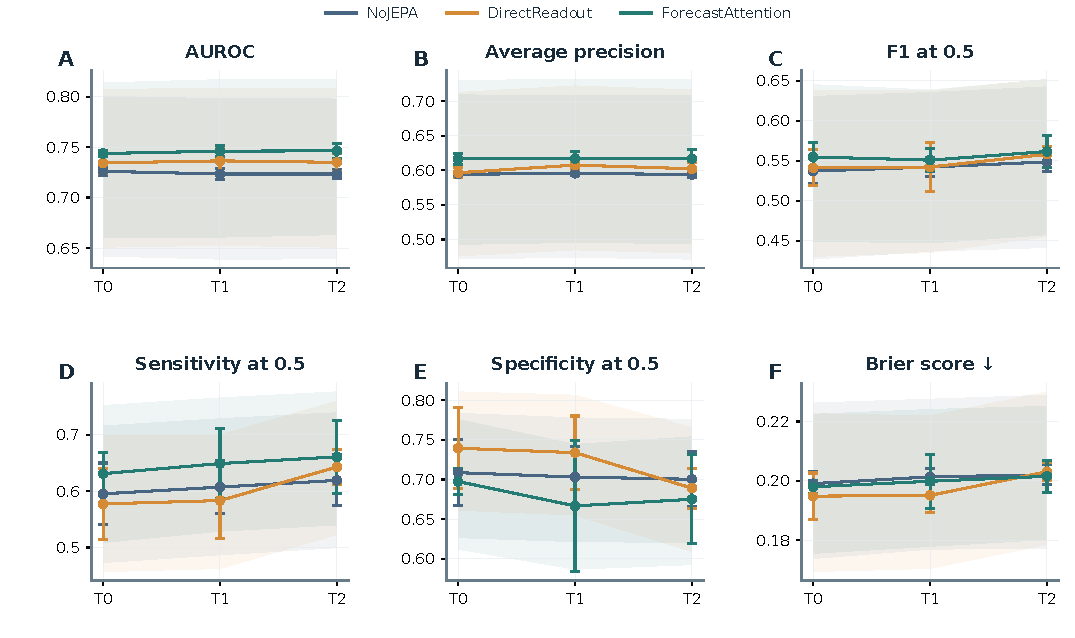
\includegraphics[width=\textwidth]{figures/landmark_performance.pdf}
\caption{Six complementary landmark summaries: AUROC, AP, F1, sensitivity, specificity, and Brier score. Metrics are computed separately from each seed's five-fold ensemble probabilities and then averaged across seeds 42, 44, and 2026. Error bars show descriptive sample seed standard deviations, while shading gives conditional 95\% shared-patient-bootstrap intervals for the seed mean. The same 175 patients appear at every seed and landmark.}
\label{fig:longitudinal}
\end{figure*}

\begin{figure*}[t]
\centering
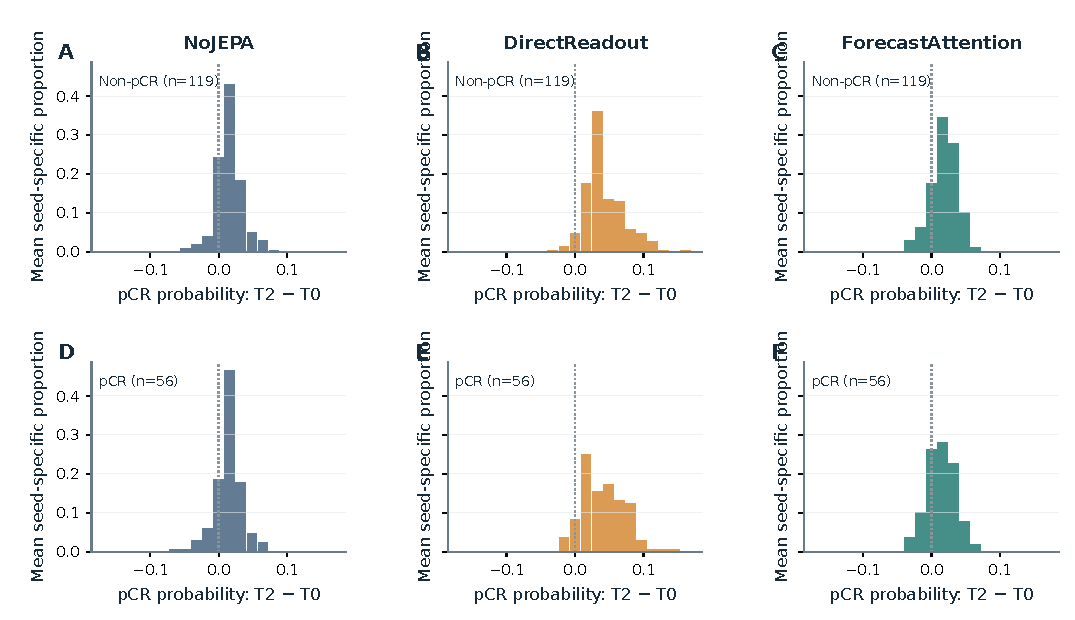
\includegraphics[width=\textwidth]{figures/outcome_score_changes.pdf}
\caption{Outcome-conditioned changes in predicted pCR probability from T0 to T2. For each seed-specific five-fold ensemble, every patient contributes one probability change. Histograms summarize these within-seed changes and are then equally averaged across seeds; probabilities are not averaged across seeds before constructing a change distribution. Panels separate models and outcome classes. Repeated seed predictions are correlated observations of the same 175 patients and do not triple the sample size. Score changes do not establish individual treatment effects.}
\label{fig:scorechanges}
\end{figure*}

\section{Supplementary subgroup and training-probe summaries}
\begin{table*}[t]
\centering
\small
\caption{Exploratory subgroup discrimination using seeds 42, 44, and 2026. Within each seed, five fold probabilities are averaged per patient before computing AUROC; Macro averages T0--T2 AUROCs. Model entries are means $\pm$ sample SD across the three seed metrics. Paired patient-bootstrap intervals for the mean ForecastAttention minus NoJEPA difference condition on all fitted models and keep the seed set fixed. Age 50 is an exploratory reporting cutpoint. Namespace groups are parts of one clinical release, not external cohorts.}
\label{tab:subgroups}
\begin{tabular}{lrrr}
\toprule
Subgroup ($n$/pCR+) & NoJEPA & Full & $\Delta$ AUROC [95\% interval] \\
\midrule
HR+/HER2- (68/11) & 0.675 $\pm$ 0.013 & 0.709 $\pm$ 0.018 & +0.033 [+0.007, +0.065] \\
HR+/HER2+ (31/12) & 0.632 $\pm$ 0.013 & 0.649 $\pm$ 0.031 & +0.017 [-0.047, +0.086] \\
HR-/HER2+ (14/7) & 0.839 $\pm$ 0.004 & 0.875 $\pm$ 0.034 & +0.036 [-0.041, +0.147] \\
HR-/HER2- (62/26) & 0.637 $\pm$ 0.004 & 0.660 $\pm$ 0.023 & +0.022 [-0.006, +0.055] \\
Age $<$50 (90/29) & 0.667 $\pm$ 0.010 & 0.686 $\pm$ 0.003 & +0.019 [+0.002, +0.037] \\
Age $\geq$50 (85/27) & 0.783 $\pm$ 0.007 & 0.806 $\pm$ 0.010 & +0.023 [+0.002, +0.048] \\
ISPY2 namespace (125/39) & 0.679 $\pm$ 0.002 & 0.701 $\pm$ 0.003 & +0.023 [+0.006, +0.042] \\
ACRIN-6698 namespace (50/17) & 0.845 $\pm$ 0.008 & 0.860 $\pm$ 0.014 & +0.016 [-0.003, +0.035] \\
\bottomrule
\end{tabular}
\end{table*}

\begin{table*}[t]
\centering
\small
\caption{Archived epoch 20 fixed-training-probe diagnostics for seeds 42, 44, and 2026. Each entry is the mean $\pm$ sample SD of three seed-specific five-fold mean skills, distinct from probability ensembling for pCR. Skill is $1-\mathrm{L1}_{forecast}/\mathrm{L1}_{copy}$ within each snapshot\textquotesingle s EMA coordinates; positive is better than holding the landmark state constant. Forecast targets require a continuous actually observed visit chain. These are training-probe summaries, not best-checkpoint holdout forecast evaluations. NoJEPA has no trained-world diagnostic.}
\label{tab:worldprobe}
\begin{tabular}{lrrr}
\toprule
Model & Horizon 1 skill & Horizon 2 skill & Horizon 3 skill \\
\midrule
NoJEPA & -- & -- & -- \\
DirectReadout & +0.007 $\pm$ 0.022 & +0.055 $\pm$ 0.017 & +0.172 $\pm$ 0.083 \\
ForecastAttention & -0.058 $\pm$ 0.018 & -0.058 $\pm$ 0.040 & +0.009 $\pm$ 0.020 \\
\bottomrule
\end{tabular}
\end{table*}


\section{Reproducibility and reporting items to complete}
The source package includes aggregate CSV files, source-report hashes, reproducible metric and figure scripts, the shared-patient-bootstrap procedure, and the official article class. The significance CSV includes raw $p$ values, within-family Holm adjustment, and adjustment over all 90 tests as a sensitivity analysis. It contains no patient identifiers, patient-level prediction rows, original MRI volumes, or model checkpoints. The method figure includes only rendered, anonymous development-image slices. Every variant uses training seeds 42, 44, and 2026. Five fold probabilities are averaged per patient within each seed before computing pCR metrics, and seed-specific metric values are then equally averaged. Individual-fold metrics are retained for numerical audit; archived training diagnostics are summarized across folds within seed and then across seeds in their own latent coordinates.

\todo{Before submission, complete author and ethics statements; verify the precise pCR pathology definition; document codec and segmentation patient-level pretraining provenance; add matched external baselines and prospectively locked training and analysis policies; audit external-cohort independence; and confirm the journal's current submission and anonymization requirements.}
